
\section{Agent Comparisons}

For each table in this section, we compare two of the strategies discussed in the previous section. At first, we look at
teams where the two agents follow the same strategy, followed later by teams consisting of two different types of agents.
Unless otherwise noted, all the statistics were taken from a simulation of 10,001 games. In these games, it was forced
that the dealer call trump to be $\spadesuit$ for simplicity, as the agents do not have a strategy for calling trump.
This setup might be considered unfair to the dealing team, but all players share the disadvantage and aim to make the best
out of the situation they find themselves in. Given enough games, the disadvantages will even out.
Each game was played until a team had 10 points (teams can get 11 points if they score 2 points when they are at 9 points).

Each agent was also timed when making it's decisions. However, each of these made over 500,000 decisions and the slowest
agent took about 3 seconds to make all these decisions. Due to this, the timings won't be included as they are indistinguishable
during play against a human. With exception of course to the MonteCarlo agent, where each decision is given a set amount of time.


\subsection{Simple Strategies}

The simple strategies were compared to each other. Figures \ref{fig:results_low} and \ref{fig:results_random} show the results of their competition.
As to be expected, Low did poorly overall. Low managed to still win some games however, since Low essentially keeps it's highest cards for the
end of the game. When they get a lucky deal, they can manage to scrape together enough tricks to win a hand. Generally though, playing Low is
worse than playing Random. On the other hand, playing High proved to be slightly better than playing Random, though not by very much.
Also not surprising is that High beats Low, likely due to winning early tricks. Each of the simple agents perform very quickly, each performing
their decisions in very little time.

\begin{figure}[h]
    \centering
    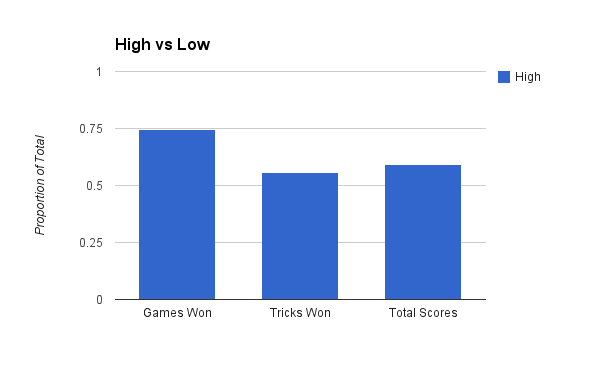
\includegraphics[scale=0.5]{data/low.png}
    \caption{Results of the Low agent against the High agent.}
    \label{fig:results_low}
\end{figure}

\begin{figure}[h]
    \centering
    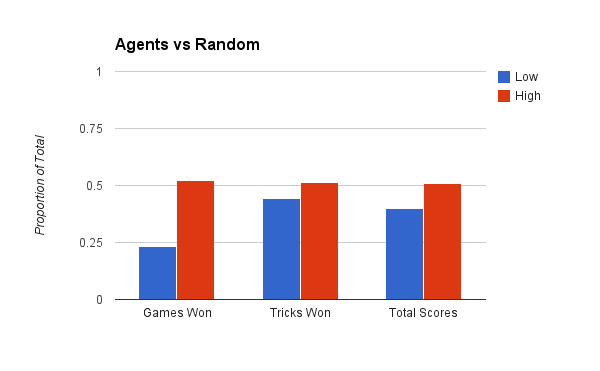
\includegraphics[scale=0.5]{data/random.png}
    \caption{Results of the Random agent against other agents.}
    \label{fig:results_random}
\end{figure}

\subsection{More Complex Strategies}

Figure \ref{fig:results_highlow} show the results for the HighLow agent against the simple strategies. The results show a staggering
favour for the HighLow agent, able to win handily against any of the simple strategies.

Figure \ref{fig:results_coophighlow} show the results for the CoopHighLow agent against the other strategies. Following the trend of 
the HighLow agent, the CoopHighLow proves to be very powerful compared to the simple strategies. This also shows the results of an
important competition. The CoopHighLow and HighLow agents both prove strong agents, but only one of the tries to cooperate with
their team mate. The results favour the CoopHighLow agent, who took on average about a point more per game.

\begin{figure}[h]
    \centering
    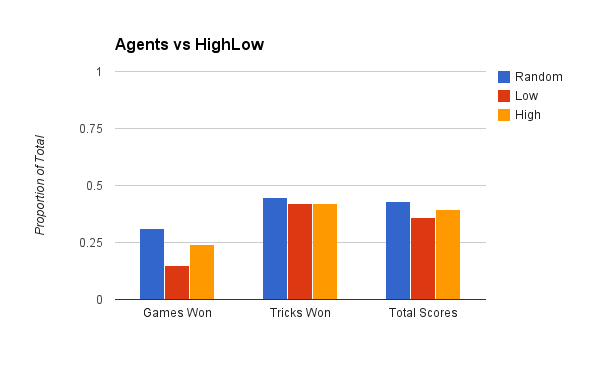
\includegraphics[scale=0.5]{data/highlow.png}
    \caption{Results of the HighLow agent against other agents.}
    \label{fig:results_highlow}
\end{figure}

\begin{figure}[h]
    \centering
    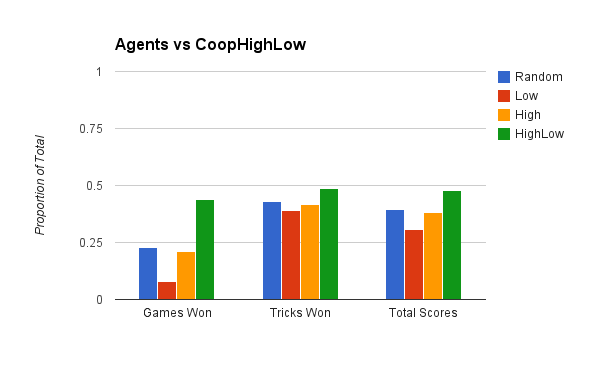
\includegraphics[scale=0.5]{data/coophighlow.png}
    \caption{Results of the CoopHighLow agent against other agents.}
    \label{fig:results_coophighlow}
\end{figure}


\subsection{Markov Decision Strategy}

Here, we show the results of two different Markov agents. They follow the same strategy, however the values they assign to each card
is different. The first agent uses the number of tricks a card wins out of all possible tricks given the current trump suit as the value for
each card. This proved to perform strangely, so an additional value base was formed. Markov2 uses a very similar value base; the value of
a card is the number of tricks the card can win which derive from the current trick and given the trump suit. This different value
base lends itself more closely to the actual values of the cards. For example, an ace that isn't the lead suit or trump cannot win any tricks,
so it should be considered a powerful card. When leading a trick, Markov2 behaves identically to Markov. Both Markov agents used a threshold $\tau$
of 0.25 due to there being 4 players in the game.

Something worth mentioning, these Markov strategies precomputed all the values of the cards and stored them for quick lookup when needed during
the games. They perform much faster this way, but used quite a bit of memory (around 1GB). However, the time taken to precompute the values
was only on the order of a second or two, so in real games they can be calculated on the fly quickly enough.

As mentioned, Markov performs strangely. Markov proves worse than Random, but slightly better than both Low and High. This is strange due to
the results shown in Figure \ref{fig:results_random}, showing that High is better than Random. When played against HighLow and CoopHighLow, Markov
did not do well at all, losing most of the games and averaging relatively low scores.

\begin{figure}[h]
    \centering
    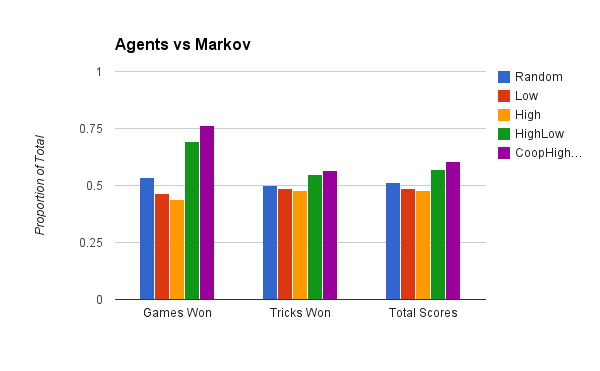
\includegraphics[scale=0.5]{data/markov.png}
    \caption{Results of the Markov agent against other agents.}
    \label{fig:results_markov}
\end{figure}

The Markov2 agent shows more promise than the Markov agent, showing it is actually slightly better than Random and still better
than both High and Low. Markov2 also is quite a bit better than the Markov agent.

This high that Markov2 experienced is quickly brought down by the soul crushing HighLow and CoopHighLow agents. Although Markov2
performed much better than Markov against these two agents, Markov2 was still trounced. Rather unfortunate.

\begin{figure}[h]
    \centering
    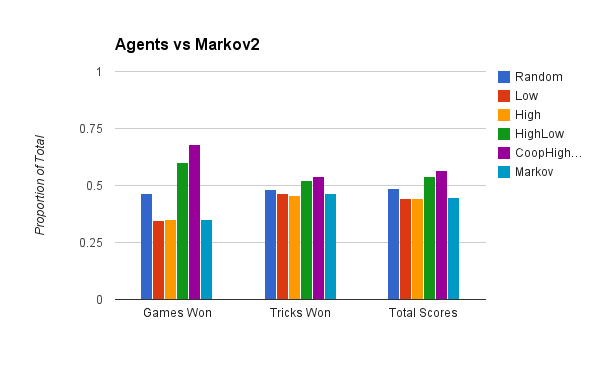
\includegraphics[scale=0.5]{data/markov2.png}
    \caption{Results of the Markov2 agent against other agents.}
    \label{fig:results_markov2}
\end{figure}


\subsection{Card Counting Strategy}

The CardCounting was modelling off of how I personally play euchre, for the most part. Human players tend to keep track of what suit
players hold and play accordingly. The CardCounting, similar to the HighLow agent, performs very well against the simple strategies.
The results are promising, as the agent achieves very high average scores in each game.


Surprisingly, the more complex strategy modelled after more human play performs not as well as expected against the relatively simple
CoopHighLow agent. CardCounting was able to beat the HighLow agent. However, against the CoopHighLow agent, the CardCounting
essentially tied, performing slightly worse but taking more tricks. It is due to this disappointing result that the Hybrid strategy
was created, in hopes to beat the CoopHighLow agent.

As shown in the previous subsection, the Markov agents are not very powerful. They are swept aside by the CardCounting agent.

\begin{figure}[h]
    \centering
    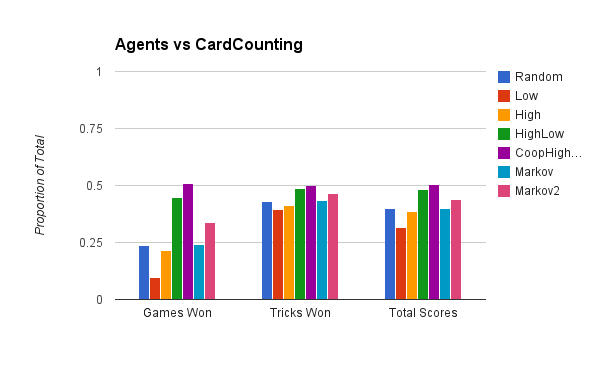
\includegraphics[scale=0.5]{data/cardcounting.png}
    \caption{Results of the CardCounting agent against other agents.}
    \label{fig:results_cardcounting}
\end{figure}


\subsection{Hybrid Strategy}

how the hybrid works


again, how disappointing


although the hybridization worked much better than cardcounting

\begin{figure}[h]
    \centering
    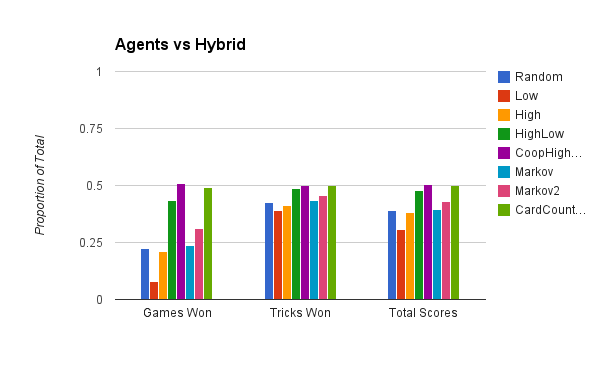
\includegraphics[scale=0.5]{data/hybrid.png}
    \caption{Results of the Hybrid agent against other agents.}
    \label{fig:results_hybrid}
\end{figure}

since markov2 worked so well, hybrid2


what is this nonsense


better than cardcounting again, worse than hybrid

\begin{figure}[h]
    \centering
    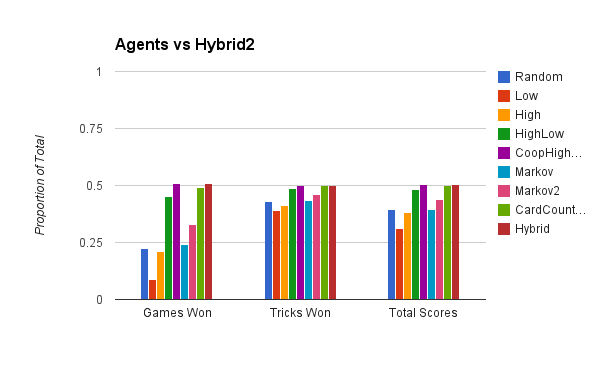
\includegraphics[scale=0.5]{data/hybrid2.png}
    \caption{Results of the Hybrid2 agent against other agents.}
    \label{fig:results_hybrid2}
\end{figure}



\subsection{Monte Carlo Agent}



\subsection{Mixed Agent Teams}

